\documentclass{scrartcl}
\setkomafont{disposition}{\normalfont\bfseries}
\usepackage[utf8]{inputenc}
\usepackage{graphicx}
\usepackage{minted}
\usemintedstyle{tango}

\title{Cybernetic Ducks}
\subtitle{Statistics 101C Lecture 4 Midterm Project Report}
\author{Ivan Escusa, Oscar Monroy, Zoe Wang,\\and Christine Marie Castle}
\date{2020-11-09}

\begin{document}

\maketitle

\section{Introduction}

Cancer is a group of diseases involving abnormal cell growth, most of which are caused by genetic mutations. Oncogenes (OG) are genes that aid in cell growth. Tumor suppressor genes (TSG) are genes that can slow cell division, repair DNA mistakes, or direct programmed cell death. The accumulation of mutations of either of these genes may result in uncontrolled cell growth and lead to cancer. Thus, it is imperative to discover cancer driver genes such as OG's and TSG's for cancer prevention, diagnosis, and treatment.

In the past few decades, scientists have identified about 250 OG's, 250 TSGs, and about 4000 neutral genes (NG), i.e. neither OG's nor TSG's, out of the 20,000 genes in the whole human genome. In recent years, many large sequencing projects, launched to catalogue genetic mutations responsible for cancer, have generated unprecedentedly large data resources. We will use statistical methods that we have learned in this course on a comprehensive gene feature data set to identify OG's and TSG's.

\section{Methodology}

\subsection{Preprocessing}

All of our cleaning was done using the \verb|tidyverse| and \verb|leaps| packages in \verb|R|. To clean the raw data set provided to us, we first checked for missing values and duplicated rows in order to replace or remove them. We found one duplicate row, which was removed, but no missing values. Next, we looked for variables with non-numeric values and luckily found that this data set has only numeric values. In particular, the \verb|id| and \verb|class| variables only consisted of integer values. After these preliminary checks, we removed the outliers, defined as observations with values more than ten standard deviations away from their respective mean, from the data set. Outliers were found to make up less than 3\% of the rows. Finally, to visually interpret differences between classes, box plots were made for each variable, split by the three classes of genes.

\subsection{Statistical Model}

For initial variable selection, we created box plots for each of the 97 potential predictors, split by the three classes of genes; we standardized the variables before plotting. We then used these box plots to assess which variables had the most pronounced differences between the three gene classes. Our motivation for this was to find predictors which had the greatest contrast between classes, as we believed those would be the most effective and efficient in differentiating the three gene classes. Additional consideration was given to the variables which showed greater potential in correctly classifying the oncogenes and tumor suppressor genes. For example, the variable \verb|N_LOF|, which represents the number of LoF (nonsense, frameshift) mutations, was initially selected based on the considerable differences in range and median among the three classes as shown in the sample of box plots in Figure \ref{fig:boxplots}.

\begin{figure}
    \centering
    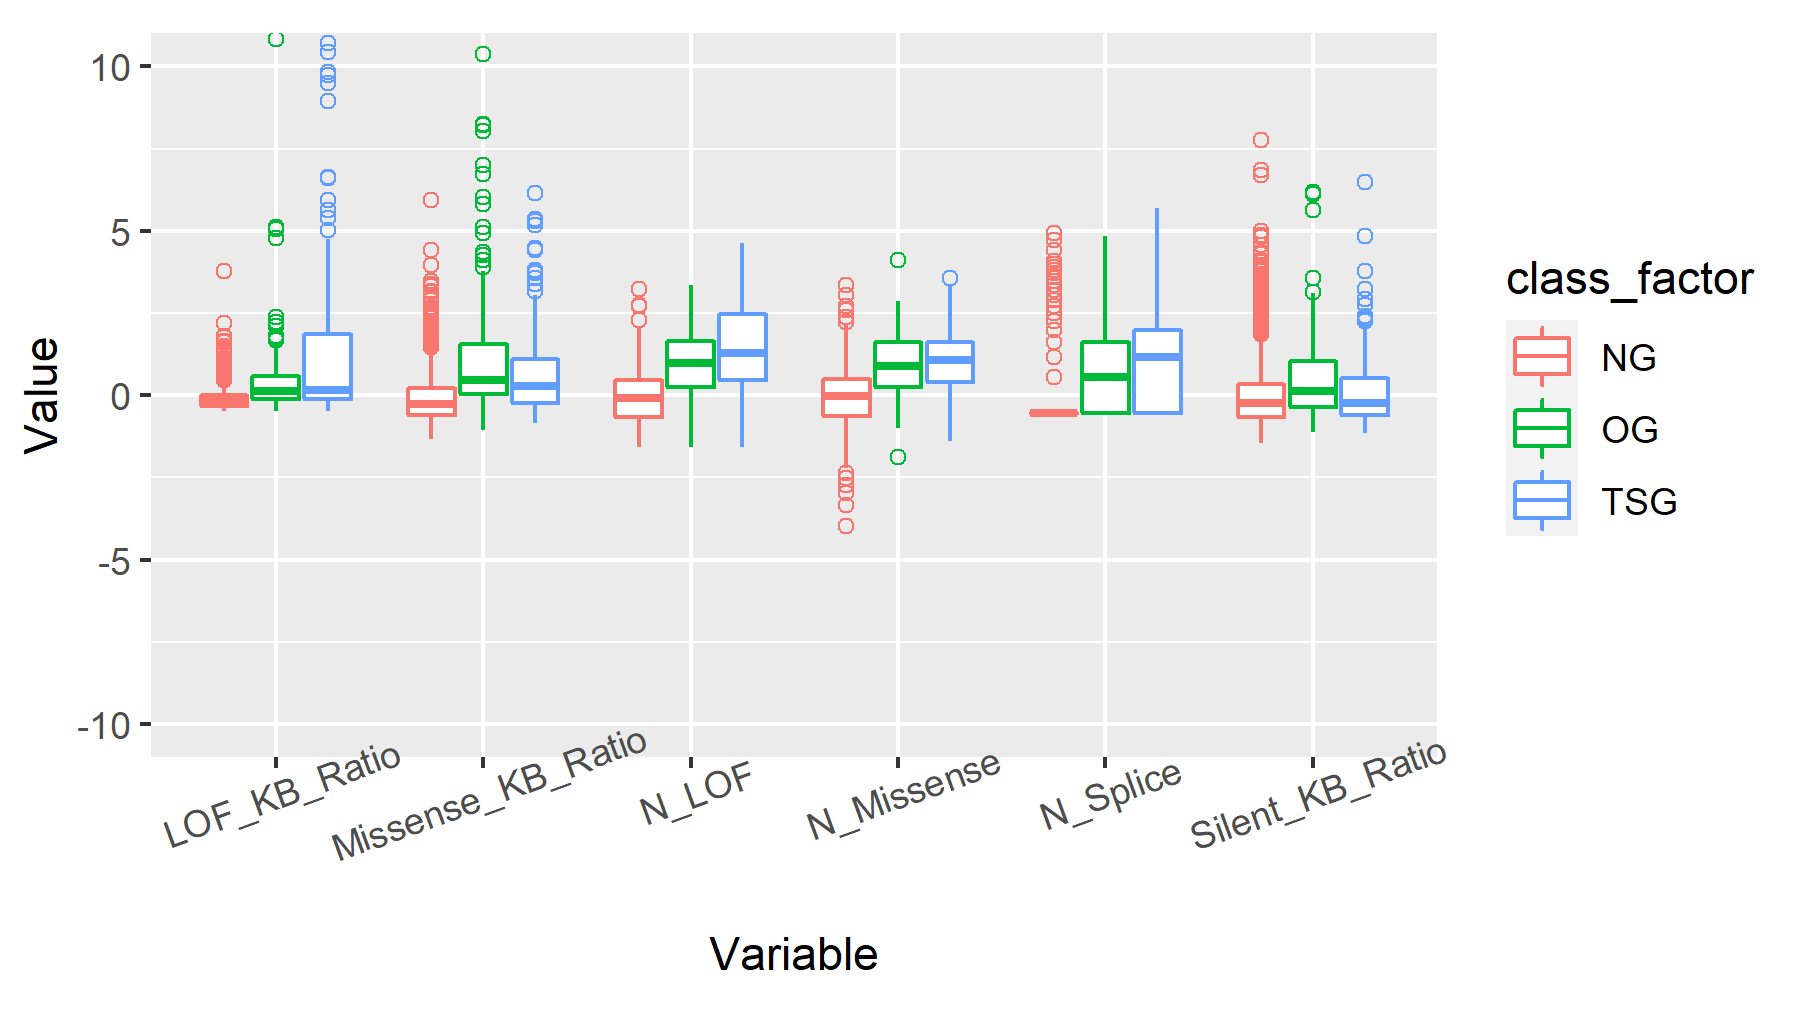
\includegraphics[width=0.75\textwidth]{boxplots.png}
    \caption{Sample of box plots used for initial variable selection}
    \label{fig:boxplots}
\end{figure}

Our model utilizes Quadratic Discriminant Analysis (QDA) to make the predictions among the three classes. We decided on the QDA method because we desired the flexibility that QDA provides as opposed to Linear Discriminant Analysis (LDA) due to the size of our data set. K-Nearest Neighbors (KNN) was also attempted, however it was consistently outperformed by QDA regardless of the value of K selected. We assessed model performance with 5-fold cross-validation. We did not consider Logistic Regression because it is not commonly used when there more than two response classes (ISLR p.137).

Next, we created an initial model for predicting the class of an unidentified gene using the predictors we identified from the box plots. To refine our predictors after the initial variable selection, we created two functions, \verb|removal_kfold_qda| and \verb|addition_kfold_qda|, that utilize for loops to cycle through variables, removing or adding them one at a time respectively. Within these loops, we used 5-fold cross-validation and calculated the average error rate, storing them in a list; this process was repeated 15 times to ensure the error rate changed significantly enough to justify adding or removing one or more variables. With that, we generated summary statistics and box plots to provide visualizations of the range and to determine if there was enough change to the predictions' viability.

\begin{figure}
    \centering
    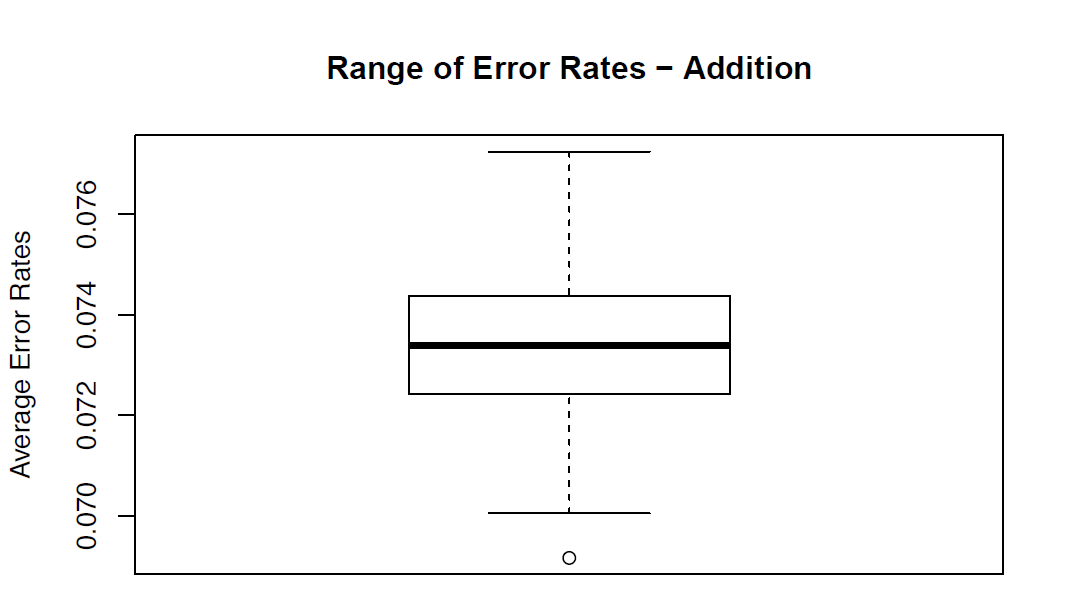
\includegraphics[width=0.75\textwidth]{removal.png}
    \caption{Box plot of average error rates produced with the removal loop}
    \label{fig:removal}
\end{figure}

Figure \ref{fig:removal} shows the box plot of the removal loop. The results display an outlier at the bottom, which indicates to us to remove the variable representing the outlier as a predictor for the model. In this way, we can lower the overall average error rate of our predictions to approximately 6.9\%. After further refining based on this process and testing through submissions to Kaggle, we settled on our final model, which features 39 of the given 97 variables as predictors.

\section{Results}

Our best evaluation metric was a Kaggle score of 0.76644.

\section{General Conclusions}

One of the reasons QDA may have worked well for this problem is because we had a large set of variables to select from. The large number of observations in the data set also mitigated the increase in variance, which allowed for more flexibility and thus a lower bias in our model. On the other hand, the model may not have worked as well as we hoped because the increase in variance was still significant enough to cause overfitting to the training data. Our model may also have suffered if the underlying assumption of QDA, that the predictors are approximately normally distributed in each of the classes, was violated. Another downfall of our model is that the methodologies used to get to the final predictions, namely the loops, are computationally expensive and required several minutes to run.

\pagebreak

\section*{Statement of Contributions}

All four members of the Cybernetic Ducks: Ivan Escusa, Oscar Monroy, Zoe Wang, and Christine Marie Castle contributed to submitting data for the Kaggle Competition as well as providing the write-up and report for our process with the best model as evaluated with Kaggle. Our team made a total of 33 submissions for this project, 25 of which were successful. For this project, each of the members contributed to different parts of the Kaggle Competition. Christine Marie Castle cleaned up the data, created the box plots, submitted one Kaggle prediction that didn't make it above the benchmark, and typeset this report. Once the data was cleaned, Oscar Monroy contributed to submitting 18 different sets of predictions and was able to improve the team's best predictions after his 2nd, 7th, 8th, 12th, and 15th submissions. Our best prediction was on his 15th successful submission, the team's 22nd successful submission, and the 29th overall prediction including ones that had errors. Ivan Escusa also contributed three submissions to the Kaggle competition, all of which were barely above the benchmark of 0.5983 and weren't effective enough. Zoe Wang contributed three submissions to Kaggle, one with a score of 0.66, which was the highest score at the time, but the other submissions were below the benchmark. All four members also contributed to the visualizations and the appendix with all of the code in the finalization of this report.

\pagebreak

\section*{Appendix}

\inputminted{R}{mt_final.R}

\end{document}
